% Hình giải thích chín ca còn lại của Bảng VII (Visual Genome), cùng cách vẽ với Hình 2.
% Hình sinh bằng report/figures/scripts/make_vg_appendix_figures.py.

\section{Hình giải thích các ca trên Visual Genome}
\label{app:vg-figures}

Phụ lục này trình bày hình giải thích của chín ca còn lại trong Bảng~\ref{tab:vg-cases}, vẽ cùng cách với Hình~\ref{fig:vg-case}. Nút cam là ảnh, nút xám là vật trong scene graph; cạnh xanh là phần tử của tập giải thích $\mathcal S$, độ dày và số trong ngoặc là $\Delta$ điểm đồ thị khi bỏ phần tử đó; $\times n$ là $n$ vật cùng tên. Với ca thất bại, hình vẽ ảnh đúng và tập giải thích của nó, như cột phần tử đóng góp lớn nhất của Bảng~\ref{tab:vg-cases}; chú thích nêu ảnh sai đứng hạng nhất dựa vào những phần tử nào.

\begin{figure*}[!t]
\centering
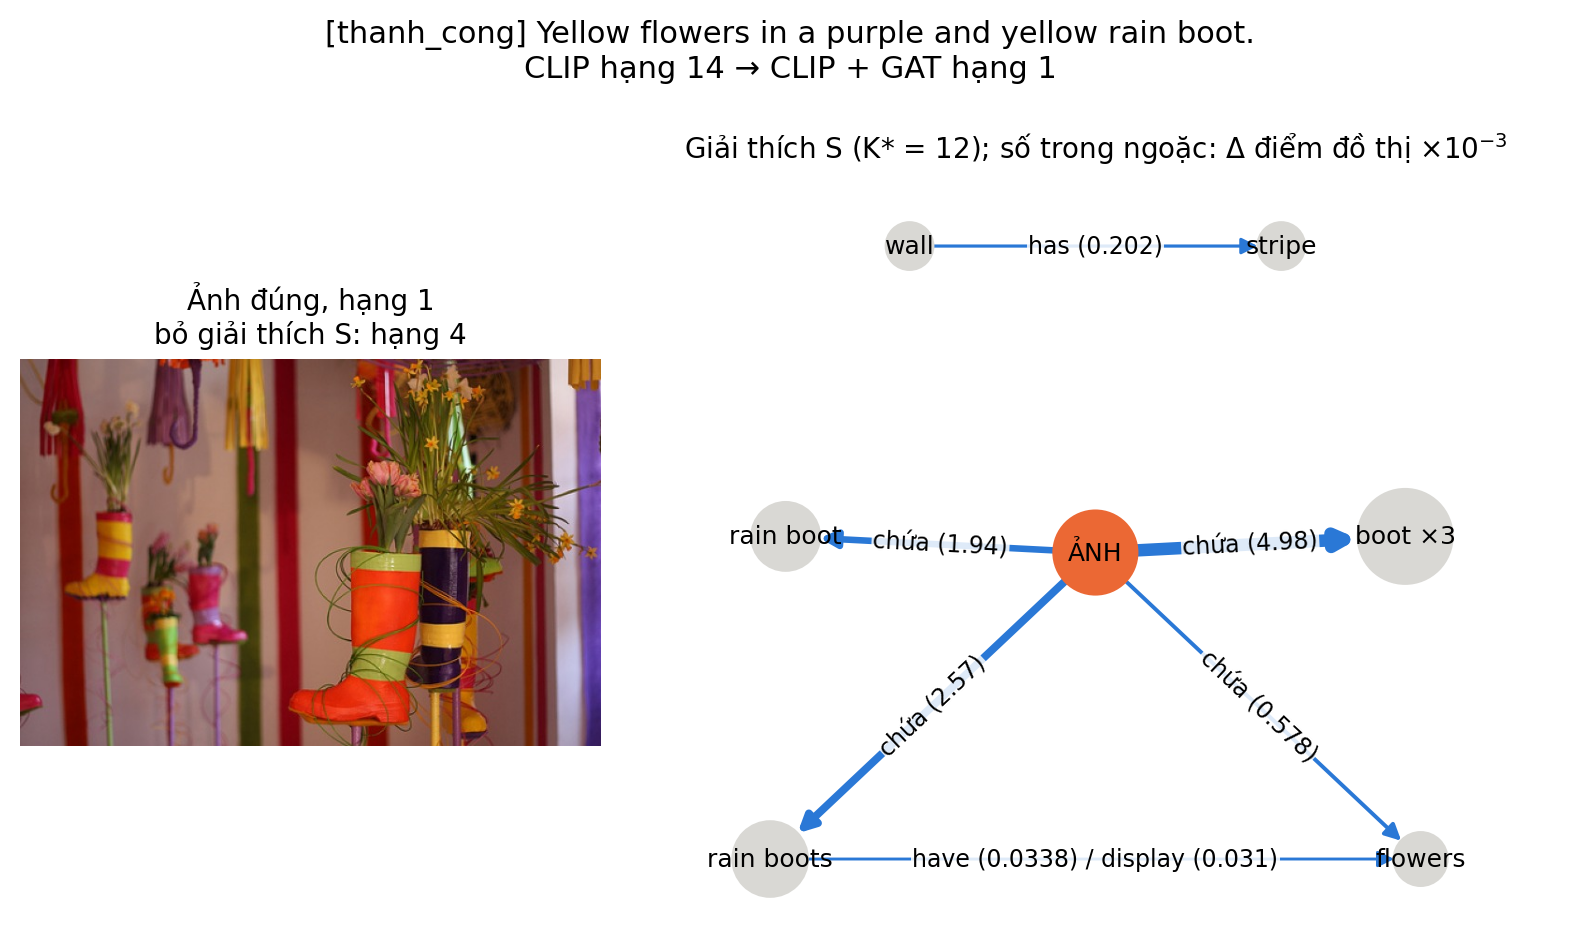
\includegraphics[width=0.78\textwidth]{figures/appendix_vg/vg_551191.png}
\caption{Ca thành công ``Yellow flowers in a purple and yellow rain boot'': CLIP hạng 14, CLIP + GAT hạng 1, bỏ tập giải thích thì ảnh về hạng 4.}
\label{fig:app-vg-rainboot}
\end{figure*}

\begin{figure*}[!t]
\centering
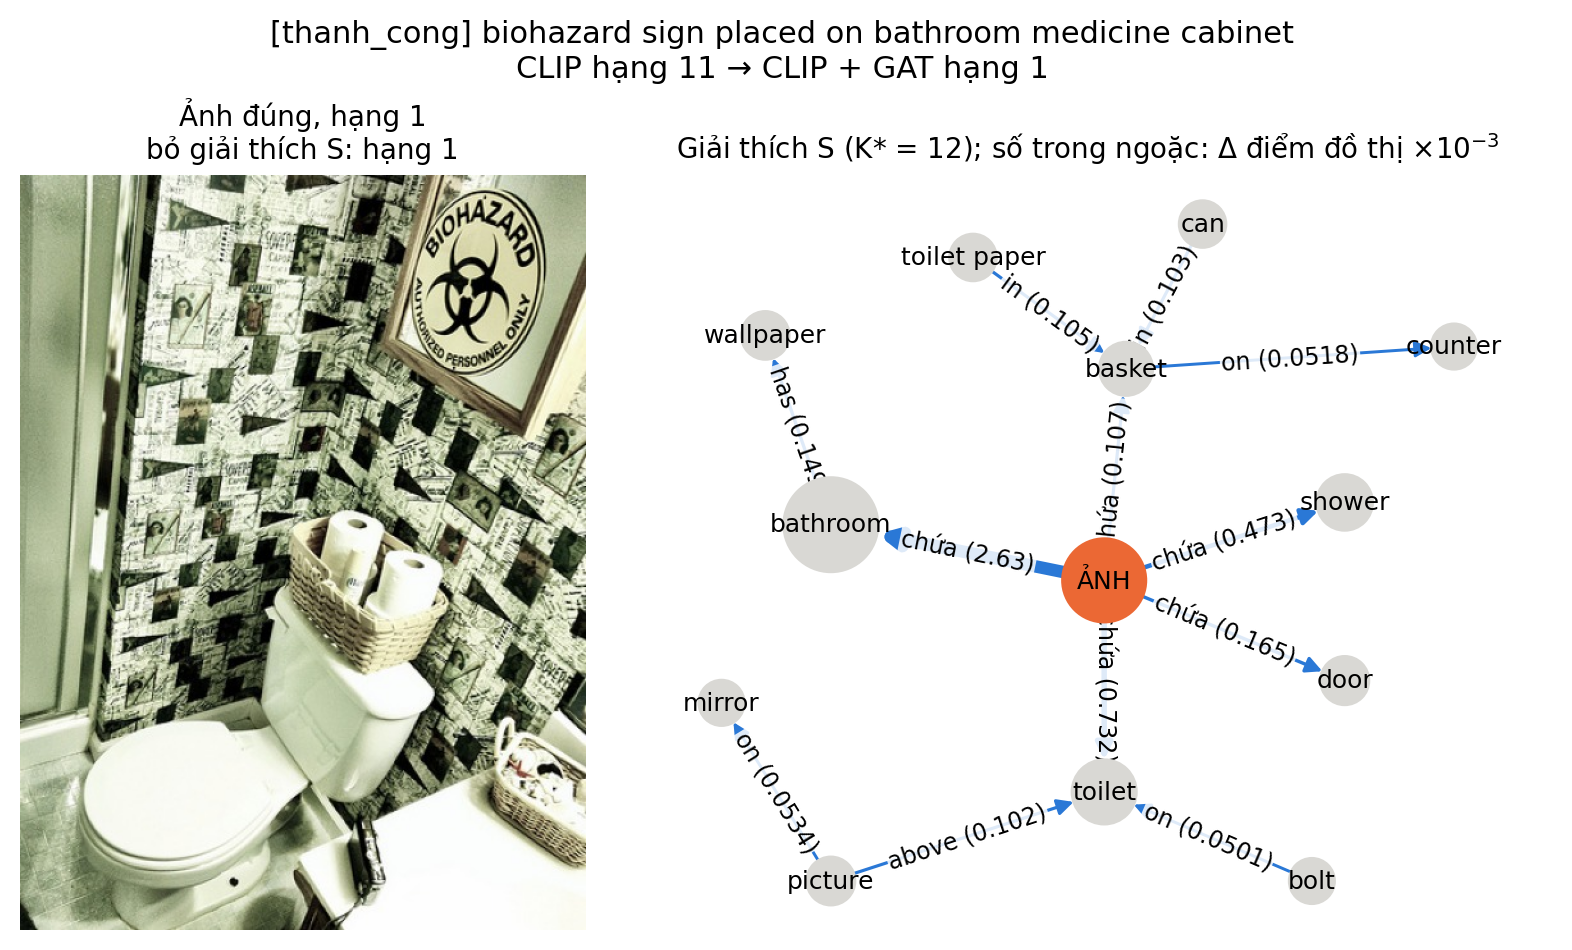
\includegraphics[width=0.78\textwidth]{figures/appendix_vg/vg_2418127.png}
\caption{Ca thành công ``biohazard sign placed on bathroom medicine cabinet'': CLIP hạng 11, CLIP + GAT hạng 1, bỏ tập giải thích ảnh vẫn ở hạng 1.}
\label{fig:app-vg-biohazard}
\end{figure*}

\begin{figure*}[!t]
\centering
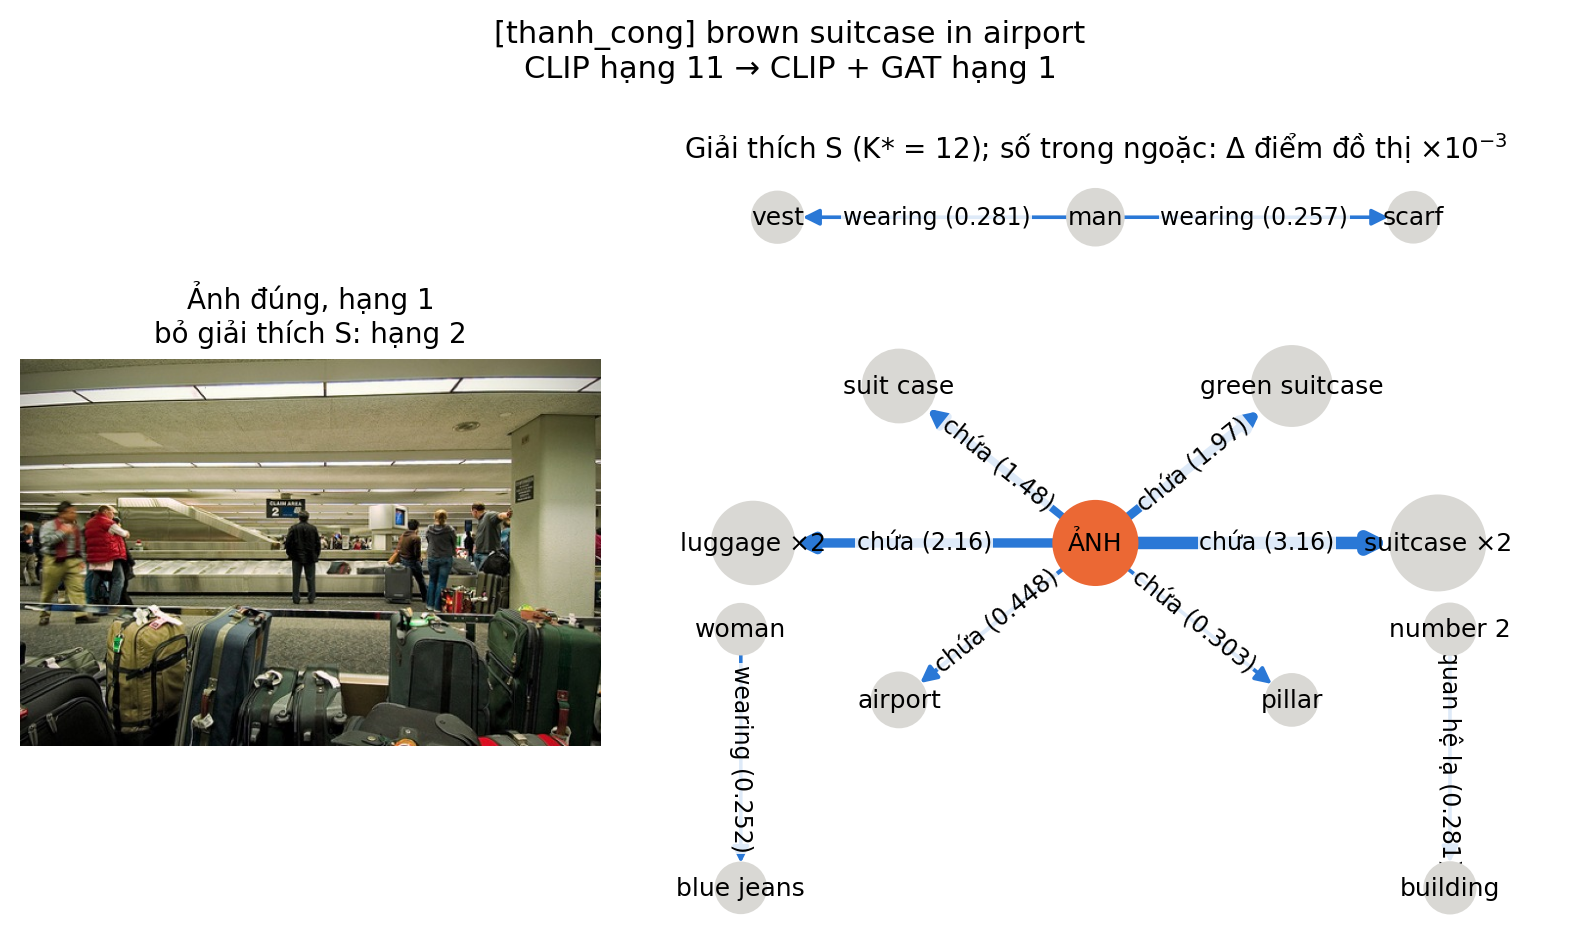
\includegraphics[width=0.78\textwidth]{figures/appendix_vg/vg_2138299.png}
\caption{Ca thành công ``brown suitcase in airport'': CLIP hạng 11, CLIP + GAT hạng 1, bỏ tập giải thích thì ảnh về hạng 2.}
\label{fig:app-vg-suitcase}
\end{figure*}

\begin{figure*}[!t]
\centering
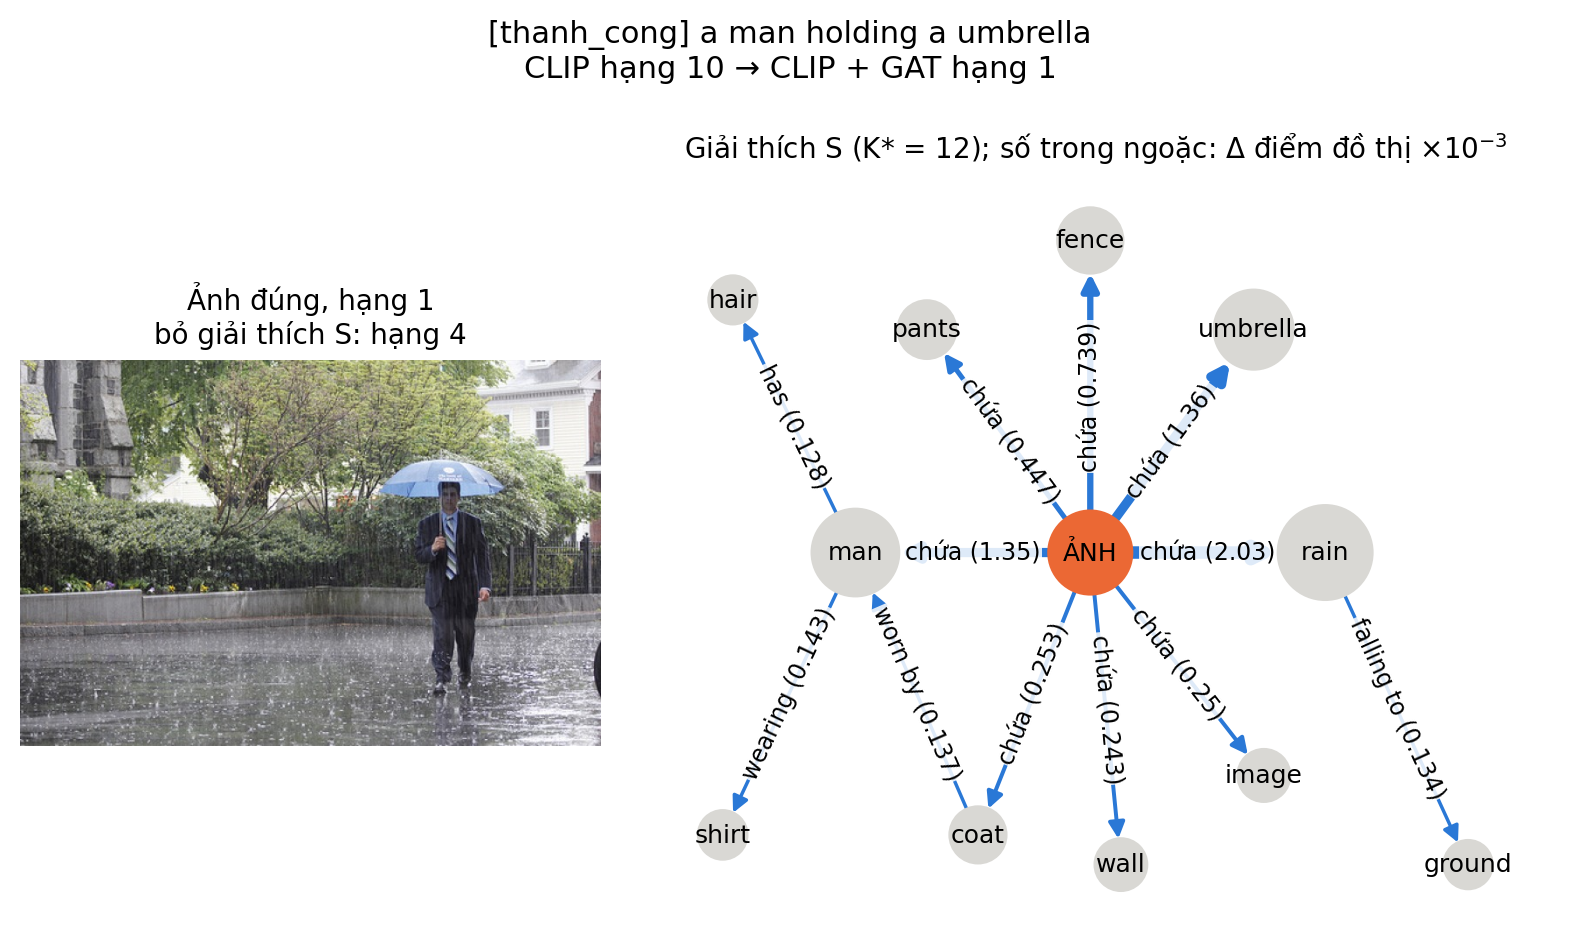
\includegraphics[width=0.78\textwidth]{figures/appendix_vg/vg_4608567.png}
\caption{Ca thành công ``a man holding a umbrella'': CLIP hạng 10, CLIP + GAT hạng 1, bỏ tập giải thích thì ảnh về hạng 4.}
\label{fig:app-vg-umbrella}
\end{figure*}

\begin{figure*}[!t]
\centering
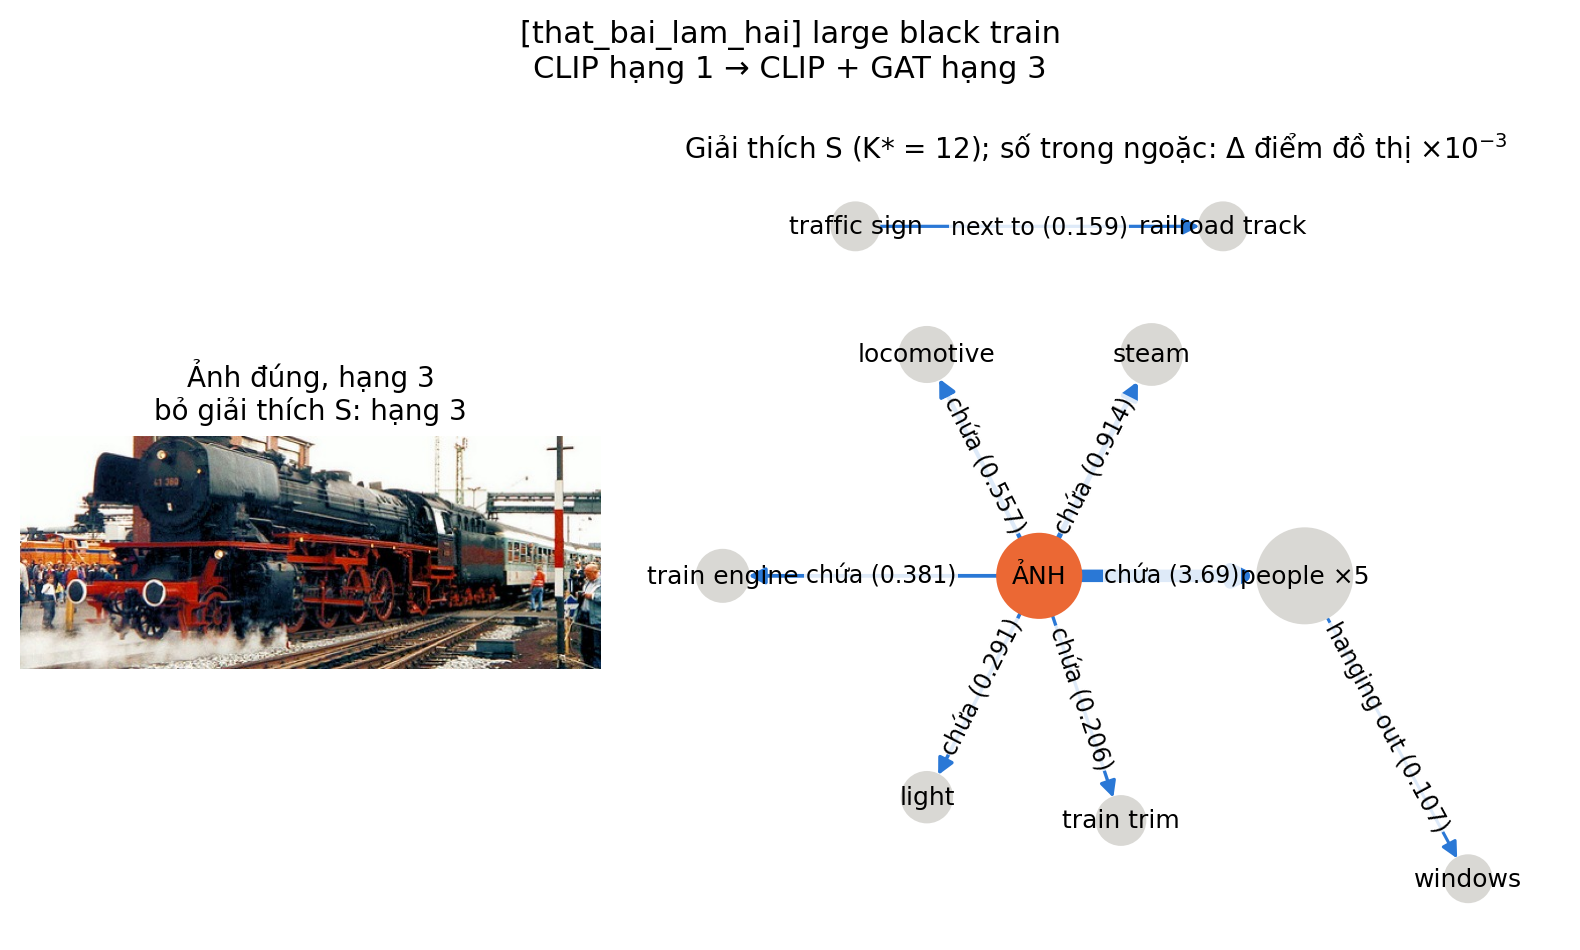
\includegraphics[width=0.78\textwidth]{figures/appendix_vg/vg_1317304.png}
\caption{Ca thất bại ``large black train'': CLIP hạng 1, CLIP + GAT hạng 3; bỏ tập giải thích của ảnh đúng thì ảnh vẫn ở hạng 3. Ảnh sai đứng hạng 1 dựa vào \textit{smoke stack}, \textit{steam} và \textit{smoke}; bỏ tập giải thích của ảnh sai thì nó về hạng 3.}
\label{fig:app-vg-train}
\end{figure*}

\begin{figure*}[!t]
\centering
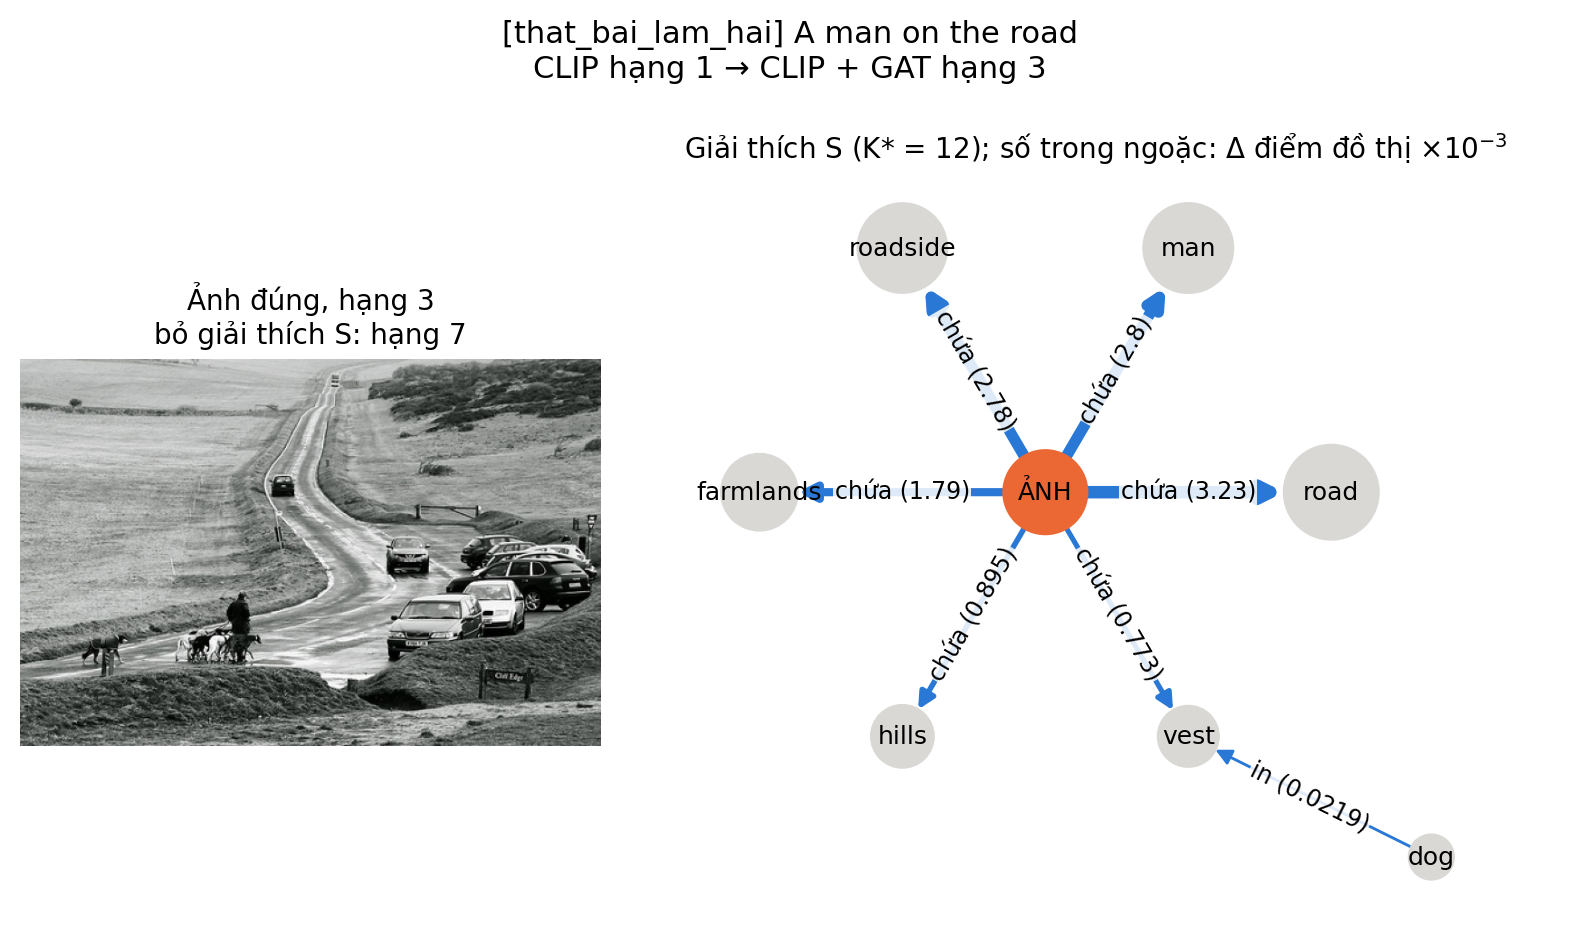
\includegraphics[width=0.78\textwidth]{figures/appendix_vg/vg_3658532.png}
\caption{Ca thất bại ``A man on the road'': CLIP hạng 1, CLIP + GAT hạng 3; bỏ tập giải thích của ảnh đúng thì ảnh về hạng 7. Ảnh sai đứng hạng 1 dựa vào \textit{road}, \textit{man} và \textit{rain}; bỏ tập giải thích của ảnh sai thì nó về hạng 2.}
\label{fig:app-vg-road}
\end{figure*}

\begin{figure*}[!t]
\centering
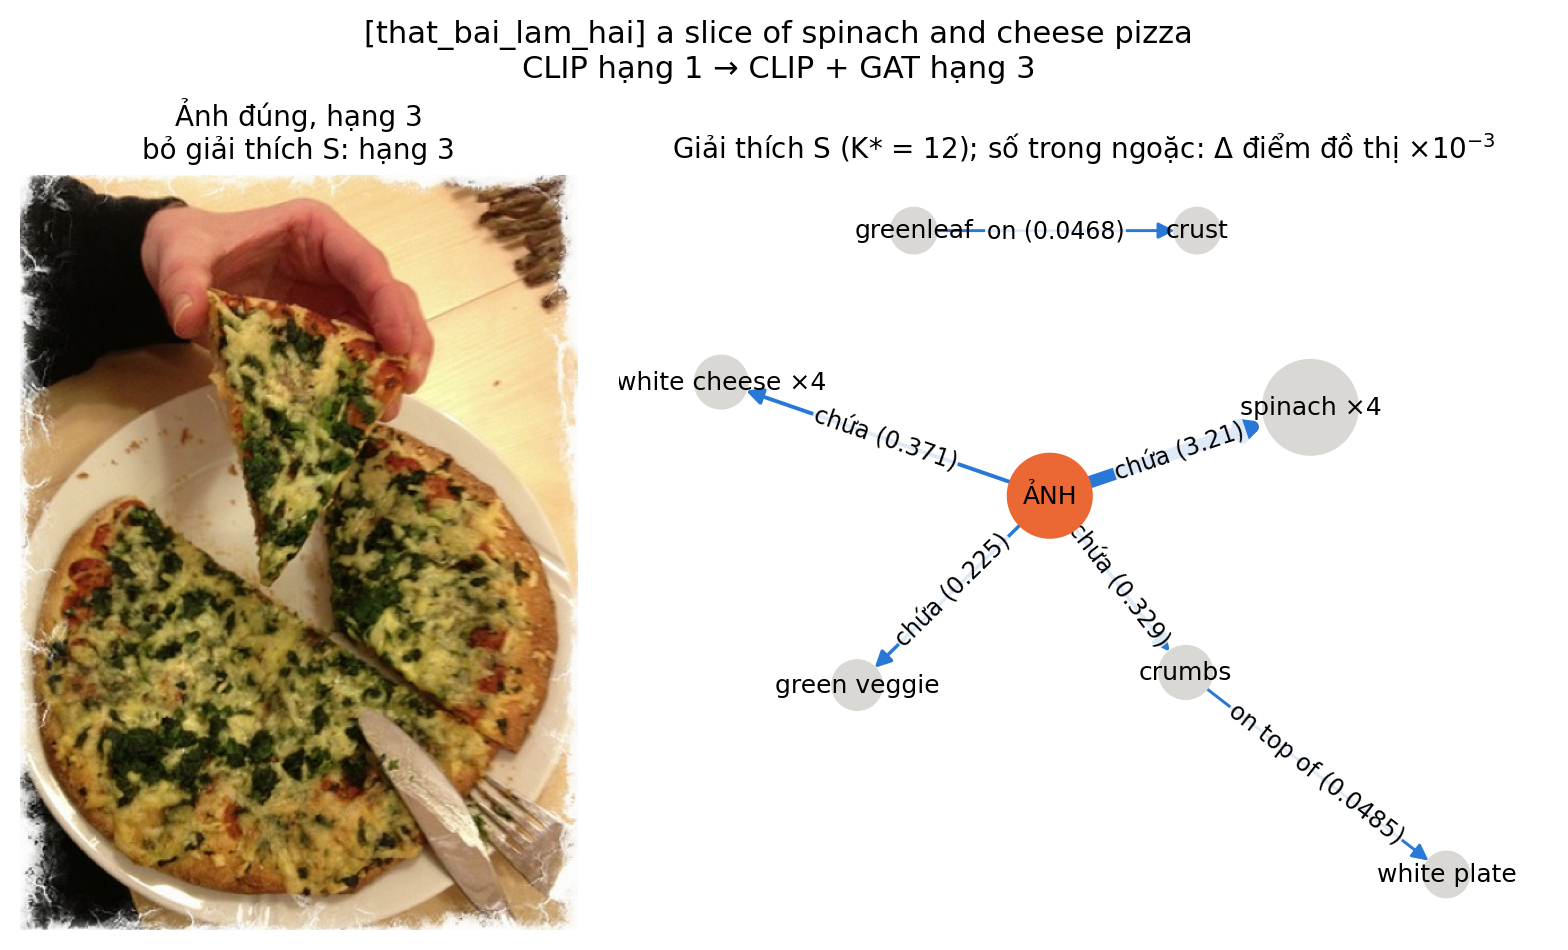
\includegraphics[width=0.78\textwidth]{figures/appendix_vg/vg_3650395.png}
\caption{Ca thất bại ``a slice of spinach and cheese pizza'': CLIP hạng 1, CLIP + GAT hạng 3; bỏ tập giải thích của ảnh đúng thì ảnh vẫn ở hạng 3. Ảnh sai đứng hạng 1 dựa vào \textit{spinach} $\times2$ ($1.39\times10^{-3}$ mỗi cạnh, cao hơn $0.80\times10^{-3}$ ở ảnh đúng) và \textit{doorway} $\times3$; bỏ tập giải thích của ảnh sai thì nó vẫn ở hạng 1.}
\label{fig:app-vg-pizza}
\end{figure*}

\begin{figure*}[!t]
\centering
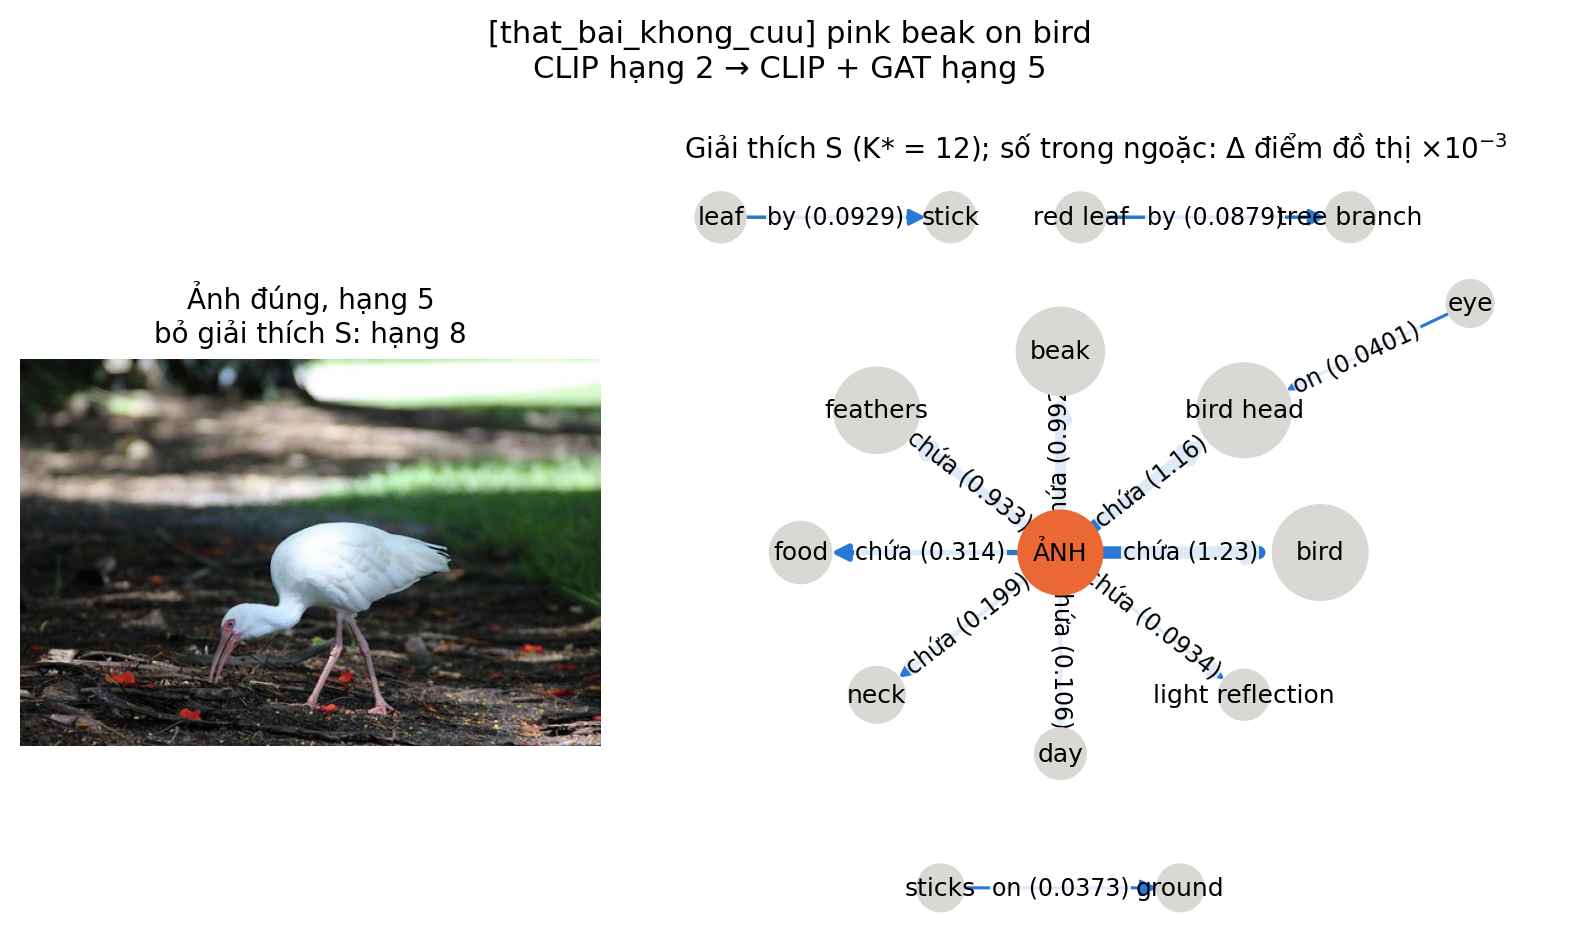
\includegraphics[width=0.78\textwidth]{figures/appendix_vg/vg_2000339.png}
\caption{Ca thất bại ``pink beak on bird'': CLIP hạng 2, CLIP + GAT hạng 5; bỏ tập giải thích của ảnh đúng thì ảnh về hạng 8. Ảnh sai đứng hạng 1 là đàn hồng hạc, dựa vào \textit{flamingo} $\times3$, \textit{beak} $\times2$ và \textit{bird}; bỏ tập giải thích của ảnh sai thì nó vẫn ở hạng 1.}
\label{fig:app-vg-beak}
\end{figure*}

\begin{figure*}[!t]
\centering
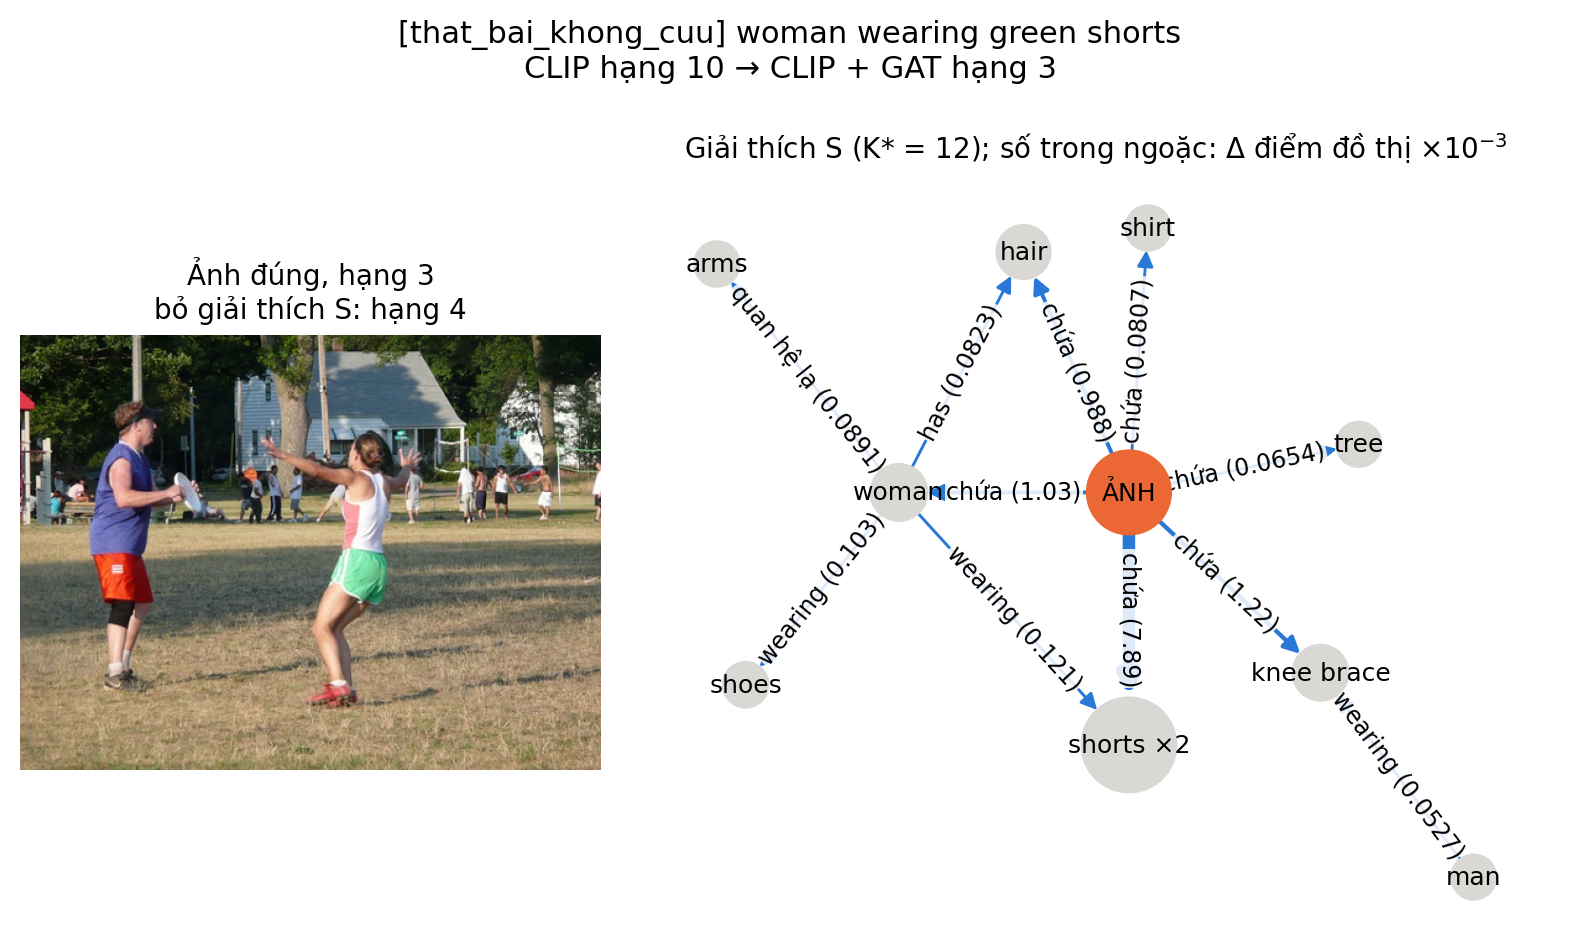
\includegraphics[width=0.78\textwidth]{figures/appendix_vg/vg_1939039.png}
\caption{Ca thất bại ``woman wearing green shorts'': CLIP hạng 10, CLIP + GAT hạng 3; bỏ tập giải thích của ảnh đúng thì ảnh về hạng 4. Ảnh sai đứng hạng 1 dựa vào một cạnh \textit{contains shorts} ($14.9\times10^{-3}$) và \textit{vest with fringe}; bỏ tập giải thích của ảnh sai thì nó vẫn ở hạng 1.}
\label{fig:app-vg-shorts}
\end{figure*}
